%!TEX root = ../Thesis.tex

\usetikzlibrary{arrows,shapes,positioning,shadows,trees}

\usetikzlibrary{arrows}
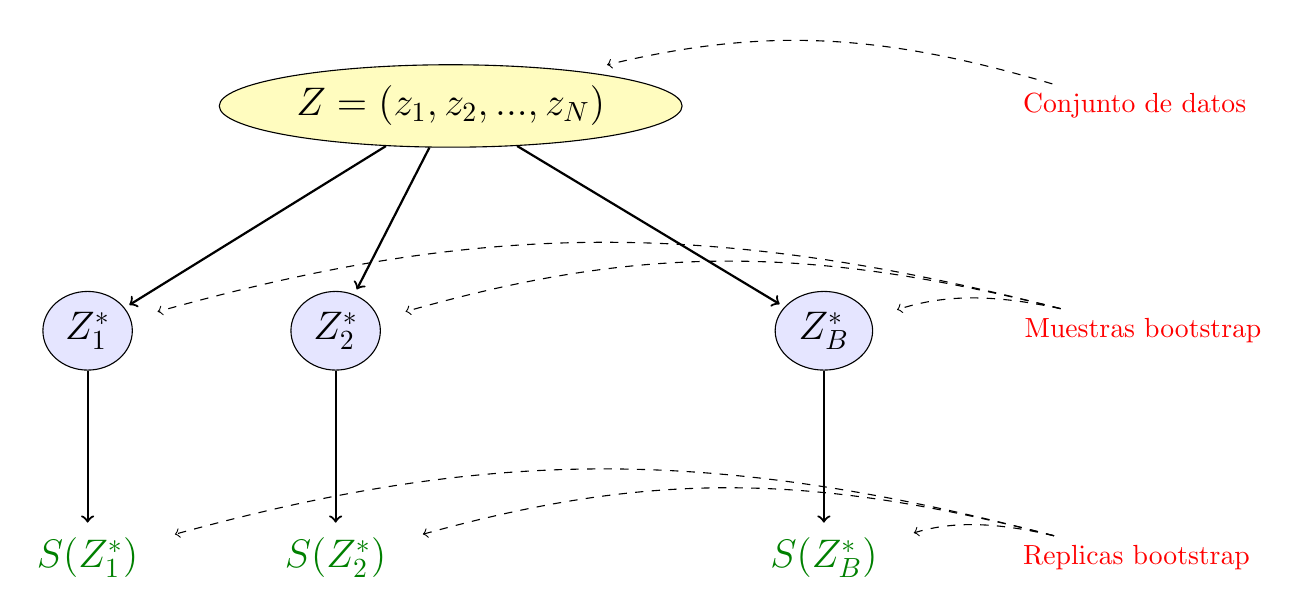
\begin{tikzpicture}[
  node distance = 1cm, auto,font=\sffamily\Large\bfseries,
  % STYLES
  every node/.style={node distance=3cm},
  % OWNs
  znode/.style={ellipse,fill=blue!10,draw},
  snode/.style={draw=none,fill=none,text=black!50!green},
  comme/.style={draw=none,fill=none,text=red,font=\normalsize}]

  \node[znode, fill=yellow!25] (main) {$Z = (z_1, z_2, ..., z_N)$};
  	\node[znode] [below left={3cm} of main](z1) {$Z^{*}_1$};
    \node[znode] [right=2cm of z1](z2) {$Z^{*}_2$};
    \node[znode] [right=5cm of z2](zb) {$Z^{*}_B$};
    
  \node[snode] [below=2cm of z1](sz1) {$S(Z^{*}_1)$};
  \node[snode] [below=2cm of z2](sz2) {$S(Z^{*}_2)$};
  \node[snode] [below=2cm of zb](szb) {$S(Z^{*}_B)$};
  
  \node[comme] [right=4.2cm of main](c1) {Conjunto de datos};
  \node[comme] [right=1.8cm of zb](c2) {Muestras bootstrap};
  \node[comme] [right=1.6cm of szb](c3) {Replicas bootstrap};
  
  \path[->,thick,shorten >=2pt]
    (main) edge (z1)
  	(main) edge (z2)
	  (main) edge (zb)
  	(z1) edge (sz1)  
    (z2) edge (sz2)  
    (zb) edge (szb);
    
  \path[dashed, ->, thin, bend right=15, shorten >= 10pt]
  	(c1) edge (main)
    (c2) edge (z1)
    (c2) edge (z2)
    (c2) edge (zb)
  	(c3) edge (sz1)
    (c3) edge (sz2)
    (c3) edge (szb);  
\end{tikzpicture}